
\chapter{Platform description}
\section{Humanoid robot TEO}
El robot humanoide RH-2, también conocido como TEO (Task Environment Operator), de la Universidad Carlos III de Madrid, es una versión avanzada de los humanoides RH-0 y RH-1. 

El RH-2 tiene una altura de 165cm que supera los 150cm del RH-1 y los 120cm del RH-0. Su peso es de, aproximadamente , 60 kg y se estima que puede soportar objetos de hasta 2kg.

Cuenta con 24 GDL (26 GDL teniendo en cuenta los motores de la cabeza), los cuales son 3 grados más que las anteriores versiones de RH. En la Figura \ref{ref:gdl} se muestran los grados de libertad del robot, además del el tipo de movimiento que realiza cada uno, siendo 6 GDL para cada pierna, 6 GDL para cada brazo, 2 GDL en el torso y 2 GDL en la cabeza.

\begin{figure}[!hbt]
\centering
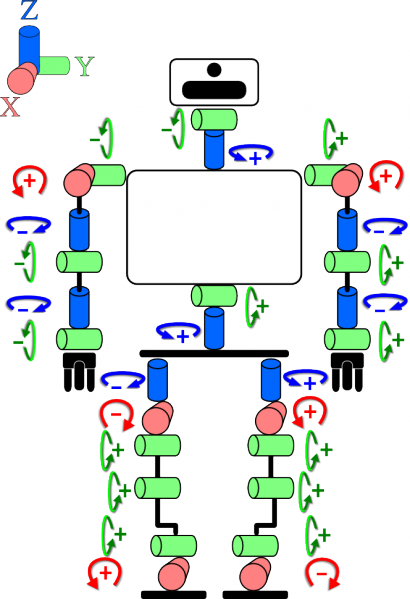
\includegraphics[scale=0.45]{teo_gdl.png}
\caption{Distribución de grados de libertad del robot TEO.}
\label{fig:gdl}
\end{figure}

El robot consta de 4 microprocesadores, uno encargado de la locomoción, otro encargado de la manipulación, otro encargado de realizar las tareas de visión artificial y por último, un procesador central que gestiona el resto. El procesador encargado de la locomoción, que controla las piernas y el torso, se encargará de procesar la información de los sensores para lograr que el robot mantenga y el equilibrio, y por consiguiente, realize una caminata estable. Por su parte el procesador manipulador se encargará de contolar el movimiento de los brazos y de la cabeza. El procesador encargado de la visión por computador opera utilizando una cámara con sensor infrarrojo ASUS incorporada en la cabeza.

El sistema de comunicaciones sigue el protocolo CAN-bus realizando una división sagital y transversal del humanoide, existiendo 4 líneas de CAN-bus. Una línea CAN se encargará de comunicar el brazo izquierdo, mientras que otra se ocupará del lado derecho. Igualmente, en el tren inferior, una línea can se ocupará de la pierna izquierda y otra de la pierna derecha.\\

A su vez, para realizar la adquisición de datos de los sensores de Fuerza-Par que lleva incorportados en los tobillos -y que serán utilizados para realizar una caminata estable-, se utilizan tarjetas de adquisición de datos PCI que trabajan en tiempo real. Con un sensor en cada tobillo, el robot dispone de dos tarjetas PCI en el procesador del tren inferior. Del mismo modo, para las tareas de manipulación se utiliza un sensor Fuerza-Par en cada muñeca conectados a través de una PCI con el procesador del tren superior.

La dotación de sensorización de fuerzas y momentos es una importante diferencia respecto a los antecesores del robot RH-2. La utilización de estos sensores, permite cerrar el bucle de control -y así, obtener realimentación-, que tan necesario es para realizar una caminata estable.


\section{Force/Torque sensors}
Los sensores Fuerza-Par (F/T) utilizados están basados en sensores extensiométricos dispuestos de tal forma que permiten obtener medidas de fuerza y momentos en los tres ejes del espacio tridimensional.

Los sensores de los que dispone el robot son los sensores comerciales JR3 descritos en la Tabla \ref{table:sensores}. Obsérvese la diferencia de fondo de escala de los sensores utilizados en las articulaciones de los tobillos a los de las muñecas. Los sensores de los tobillos tienen que ser capaces de soportar fuerzas y momentos mucho mayores incluyendo las que ejerce el propio cuerpo del robot.

\begin{table}[!hbt]
\centering
\begin{tabular}{|c|c|c|c|c|}
\hline
Articulación & Modelo & $F_{x,y}$ & $F_z$ & $M_{x,y,z}$\\
\hline
Muñecas & 50M31A & 100N & 200N & 5 Nm\\ 
\hline
Tobillos & 85M35A & 250N & 500N & 212Nm\\
\hline
\end{tabular}
\caption{Modelos y características de sensores F/T del robot. \textit{Fuente: JR3 Inc.}}
\label{table:sensores}
\end{table}

Según el fabricante, los dos primeros dígitos del modelo indican el diámetro del sensor, la letra que les sigue la serie, y los dos siguiente dígitos el espesor del mismo. De ahí, los sensores de los tobillos tendrán un diámetro de 85mm, un espesor de 35mm y es de la serie M. 

Los sensores M incluyen electrónica interna para filtrar el ruido, salida digital para la utilización de una tarjeta de adquisición de datos PCI del mismo fabricante y opción de salida analógica. La exactitud nominal de todos los sensores de esta serie es del 1\% de fondo de escala, y una resolución de 1/4000 del fondo de escala.
